\documentclass[11pt]{amsart}
\usepackage[margin=1in]{geometry}
\usepackage{amsmath,amssymb,amsthm,mathtools}
\usepackage{enumitem,booktabs,array,multirow}
\usepackage[dvipsnames]{xcolor}
\usepackage{tikz}
\usetikzlibrary{arrows.meta,calc,positioning,shapes.geometric}
\usepackage[hyphens]{url}
\usepackage[hidelinks]{hyperref}

\newtheorem{theorem}{Theorem}[section]
\newtheorem{lemma}[theorem]{Lemma}
\newtheorem{proposition}[theorem]{Proposition}
\newtheorem{corollary}[theorem]{Corollary}
\theoremstyle{definition}
\newtheorem{definition}[theorem]{Definition}
\theoremstyle{remark}
\newtheorem{remark}[theorem]{Remark}

\newcommand{\I}{\mathrel{\mathrm{I}}}
\newcommand{\nI}{\mathrel{\not\mathrel{\mathrm{I}}}}
\newcommand{\cS}{\mathcal{S}}
\newcommand{\cA}{\mathcal{A}}
\newcommand{\cD}{\mathcal{D}}
\newcommand{\cF}{\mathcal{F}}
\newcommand{\cM}{\mathcal{M}}
\newcommand{\cO}{\mathcal{O}}
\newcommand{\cP}{\mathcal{P}}
\newcommand{\cL}{\mathcal{L}}
\newcommand{\lam}{\lambda}
\newcommand{\diam}{\operatorname{diam}}
\newcommand{\new}[1]{\textcolor{BrickRed}{#1}}

\tikzset{
  pt/.style={circle,fill=black,inner sep=1.6pt},
  ln/.style={rectangle,fill=black,inner sep=2.1pt},
  npt/.style={circle,fill=BrickRed,inner sep=1.7pt},
  nln/.style={rectangle,fill=BrickRed,inner sep=2.2pt},
  blob/.style={ellipse,draw,minimum width=1.5cm,minimum height=0.55cm,inner sep=1pt,font=\scriptsize},
  old/.style={thin,black},
  gone/.style={thin,gray,dashed},
  added/.style={thick,BrickRed},
}

\title[The constructions without coordinates]{Adding points and lines to generalized polygons:\\ the constructions without coordinates}
\author{Degree--diameter lab}
\date{28 October 2026}

\begin{document}

\begin{abstract}
Written for Gabriela Araujo-Pardo and Ignacio L\'opez. Each construction of the lab is described here only in terms of incidence: points, lines, the lines through a point, the points of a line, flags, anti-flags, collinearity, distances in the incidence graph, and configurations (ovoids, spreads, $m$-ovoids, whiskers) defined by their combinatorial properties. For each construction we say what is chosen in the starting geometry, which incidences are deleted or moved, which new points and lines are added and exactly what they are incident with, which pairs of elements stop being collinear or concurrent and how the new elements repair this, and why the diameter and the degrees are as claimed. Section~\ref{sec:d3} treats the diameter-$3$ constructions in a projective plane: the three hats of Araujo-Pardo and L\'opez and our four hats, side by side and in the same words. Sections~\ref{sec:d4}--\ref{sec:d7} treat diameters $4$, $6$ and $7$ in generalized quadrangles and hexagons. The sections can be read independently.
\end{abstract}

\maketitle

\noindent\emph{Sources.} Everything here is taken from the lab's notes: \path{research/theorems/POLISHED.md} (coordinates and complete proofs of all results below), \path{research/geometry/geometry.tex}, \path{research/plus2/coords/coords.tex}, \path{research/theorems/D7_HEXAGON.md} and the joint draft \path{research/paper/joint.tex}. No new result is claimed. Every combinatorial statement in Section~\ref{sec:d3} was checked by a program that builds both structures from the rules below on a plane given only by its incidence relation (\path{research/synthetic/checks/check_d3.py}, for $q=3,4,5,7$, for the non-Desarguesian nearfield plane of order $9$, and against the coordinate version for $q\le 9$); the checks for the other sections are listed in Appendix~\ref{app:checks}.

\setcounter{section}{-1}
\section{Conventions}\label{sec:conv}

An \emph{incidence structure} consists of points, lines and a symmetric incidence relation $\I$ between points and lines. Points and lines are \emph{elements}. A \emph{flag} is an incident point--line pair, an \emph{anti-flag} a non-incident one. The \emph{degree} of an element is the number of elements incident with it. Two distinct points are \emph{collinear} if some line contains both, and two distinct lines are \emph{concurrent} if some point lies on both. We do \emph{not} assume that two points lie on at most one line: after points and lines are added, two points may have several common lines, and two lines may have the same points.

The \emph{incidence graph} has the elements as vertices and the flags as edges; it is bipartite. Distances $d(x,y)$ and the diameter are taken in it. So two points are at distance $2$ when they are collinear, a point and a line are at distance $3$ when they form an anti-flag and some point of the line is collinear with the point, and so on.

A \emph{generalized $n$-gon} is an incidence structure whose incidence graph has diameter $n$ and girth $2n$; elements at distance $n$ are \emph{opposite}. It has \emph{order $(s,t)$} if every line has $s+1$ points and every point is on $t+1$ lines. Projective planes are the generalized $3$-gons, generalized quadrangles the $4$-gons, generalized hexagons the $6$-gons. Write $n_b(\Delta,D)$ for the largest number of elements of an incidence structure with all degrees at most $\Delta$ and diameter at most $D$ (the bipartite degree--diameter problem). A generalized $n$-gon of order $(q,q)$ attains the counting (Moore) bound for $n_b(q+1,n)$. For degree $q+2$ there is no such object when $q+1$ is not a prime power, and every construction below starts from a generalized polygon of order $(q,q)$ (or $(q-1,q+1)$), and adds points and lines so that the maximum degree becomes $q+2$ (or more) while the diameter stays the same.

Distances can be read off from collinearity alone:

\begin{lemma}[Diameter in incidence terms]\label{lem:diam}
Let $\cS$ be an incidence structure in which every element is incident with at least one element.
\begin{enumerate}[label=\textup{(\alph*)}]
\item $\diam\cS\le 3$ if and only if any two points are collinear and any two lines are concurrent.
\item $\diam\cS\le 4$ if and only if for every anti-flag $(p,L)$ some point of $L$ is collinear with $p$.
\item $\diam\cS\le 6$ if and only if for every anti-flag $(p,L)$ some point of $L$ is at distance at most $4$ from $p$.
\item $\diam\cS\le 7$ if and only if any two points, and any two lines, are at distance at most $6$.
\end{enumerate}
\end{lemma}

\begin{proof}
For an even bound $D$: two points $p\neq p'$ are at distance at most $D$ as soon as $p$ is within $D-1$ of some line $L$ through $p'$ (if $p\I L$ the distance is $2$); two lines likewise. For an odd bound $D$: an anti-flag $(p,L)$ is within distance $D$ as soon as $p$ is within $D-1$ of some point of $L$. Distances between a point and a line are odd and distances between two points or two lines are even, which gives the converses.
\end{proof}

\section{Diameter 3: hats in a projective plane}\label{sec:d3}

Let $\Pi$ be a projective plane of order $q$: any two points are on exactly one line, any two lines meet in exactly one point, and every element has degree $q+1$. For points $u\ne v$ we write $uv$ for the line joining them. Both constructions in this section keep all points and lines of $\Pi$, delete or move a few flags near a chosen anti-flag, and add a few points and lines. By Lemma~\ref{lem:diam}(a) the diameter stays $3$ exactly when any two points remain collinear and any two lines remain concurrent; this is what has to be checked.

\subsection{The frame}\label{ssec:frame}
Fix an anti-flag $(A,\ell)$. Every line through $A$ meets $\ell$ in one point, and every point of $\ell$ is on one line through $A$. So the $q+1$ flags $(X,AX)$, $X$ a point of $\ell$, are the only incidences between the points of $\ell$ and the lines through $A$, and they match the points of $\ell$ with the lines through $A$. Both constructions change only some of these $q+1$ flags.

Choose distinct \emph{marked} points $X_s$ on $\ell$, indexed by a label set $S$, and put
\[
\lam_s = AX_s \qquad (s\in S).
\]
One label $a\in S$ is distinguished, and $T=S\setminus\{a\}$. We write
\[
\ell^* = \{\text{points of } \ell\}\setminus\{X_t : t\in T\},\qquad \Lambda^* = \{\text{lines through } A\}\setminus\{\lam_t: t\in T\}.
\]
So $\ell^*$ contains $X_a$ and the $q+1-|S|$ unmarked points of $\ell$, and $\Lambda^*$ contains $\lam_a$ and the $q+1-|S|$ lines joining $A$ to them. We call $A$, $\ell$, the $X_s$ and the $\lam_s$ the \emph{frame}.

\begin{itemize}[leftmargin=1.5em]
\item The construction of Araujo-Pardo and L\'opez \cite{AL20} (\emph{three hats}) uses three marked points: $S=\{0,1,a\}$, $T=\{0,1\}$.
\item The \emph{four hats} use four: $S=\{0,1,a,c\}$, $T=\{0,1,c\}$; this needs $q\ge 3$.
\end{itemize}
The labels $0,1,a,c$ are only names. The new elements are, for each $s\in S$, a \emph{hat point} $H_s$ and a \emph{hat line} $K_s$, and one more point $Q$ and one more line $M$.

\subsection{The two constructions}\label{ssec:defs}
Both constructions follow the same six rules. They differ in two permutations of $T$: the \emph{links} $\pi$, a permutation of $T$ without fixed points, and the \emph{rotation} $\rho$.

\begin{definition}\label{def:hats}
The incidence structure $\cS$ has as points the points of $\Pi$, the point $Q$ and the hat points $H_s$; as lines the lines of $\Pi$, the line $M$ and the hat lines $K_s$; and exactly the following incidences.
\begin{enumerate}[label=\textup{(R\arabic*)},leftmargin=3em]
\item\label{r:plane} The incidences of $\Pi$, except the flags $(X_s,\lam_s)$, $s\in S$; and the flags $(X_t,\lam_{\rho(t)})$, $t\in T$.
\item\label{r:hat} $H_s$ lies on every line of $\Pi$ through $X_s$ other than $\ell$ \quad ($q$ lines, $\lam_s$ among them).
\item\label{r:hatline} $K_s$ contains every point of $\lam_s$ other than $A$ \quad ($q$ points, $X_s$ among them).
\item\label{r:M} $M$ contains the points of $\ell^*$ and every hat point $H_s$.
\item\label{r:Q} $Q$ lies on the lines of $\Lambda^*$ and on every hat line $K_s$.
\item\label{r:links} The \emph{links}: $A\I K_a$, \ $H_a\I\ell$, and $H_t\I K_{\pi(t)}$ for $t\in T$.
\end{enumerate}
\end{definition}

\begin{table}[ht]
\centering\small
\renewcommand{\arraystretch}{1.2}
\begin{tabular}{@{}>{\raggedright}p{0.17\textwidth}>{\raggedright}p{0.36\textwidth}>{\raggedright\arraybackslash}p{0.39\textwidth}@{}}
\toprule
& three hats \cite{AL20} & four hats\\
\midrule
marked points & $X_0,X_1,X_a$ & $X_0,X_1,X_a,X_c$\\
flags deleted & $(X_a,\lam_a)$ & $(X_0,\lam_0)$, $(X_c,\lam_c)$, $(X_1,\lam_1)$, $(X_a,\lam_a)$\\
flags added & none & $(X_0,\lam_c)$, $(X_c,\lam_1)$, $(X_1,\lam_0)$\\
$H_s$ lies on & \multicolumn{2}{l}{the $q$ lines through $X_s$ other than $\ell$; \ $M$; \ one link line}\\
$K_s$ contains & \multicolumn{2}{l}{the $q$ points of $\lam_s$ other than $A$; \ $Q$; \ one link point}\\
$M$ contains & the $q-1$ points of $\ell$ other than $X_0,X_1$; $H_0,H_1,H_a$ & the $q-2$ points of $\ell$ other than $X_0,X_1,X_c$; $H_0,H_1,H_a,H_c$\\
$Q$ lies on & the $q-1$ lines through $A$ other than $\lam_0,\lam_1$; $K_0,K_1,K_a$ & the $q-2$ lines through $A$ other than $\lam_0,\lam_1,\lam_c$; $K_0,K_1,K_a,K_c$\\
links & $A\I K_a$, $H_a\I\ell$, $H_0\I K_1$, $H_1\I K_0$ & $A\I K_a$, $H_a\I\ell$, $H_0\I K_c$, $H_c\I K_1$, $H_1\I K_0$\\
$\pi$, $\rho$ & $\pi=(0\ 1)$, $\rho=\mathrm{id}$ & $\pi=\rho=\sigma=(0\ c\ 1)$: $0\mapsto c\mapsto 1\mapsto 0$\\
new elements & $Q,H_0,H_1,H_a$; $M,K_0,K_1,K_a$ & $Q,H_0,H_1,H_a,H_c$; $M,K_0,K_1,K_a,K_c$\\
\bottomrule
\end{tabular}
\caption{The two constructions, rule by rule. With $\rho=\mathrm{id}$, rule~\ref{r:plane} deletes and restores the flags $(X_t,\lam_t)$, $t\in T$, so the three hats delete only $(X_a,\lam_a)$.}
\label{tab:rules}
\end{table}

So the three hats of \cite{AL20} are $\cS$ with $S=\{0,1,a\}$, $\pi=(0\ 1)$, $\rho=\mathrm{id}$, and the four hats are $\cS$ with $S=\{0,1,a,c\}$ and $\pi=\rho=\sigma$. Table~\ref{tab:rules} puts the two side by side, and Figure~\ref{fig:frame} shows what rule~\ref{r:plane} and the links do to the flags between $\ell$ and the lines through $A$.

\emph{Dictionary.} In \cite{AL20} the plane is described from a flag $(P,L)$ (the point and line at infinity); $P_0$ is a point of $L$ other than $P$, and $L_0$ a line through $P$ other than $L$. In our names $P_0=A$, $L_0=\ell$, $(0,s)=X_s$, $[0,s]=\lam_s$, $Q_0=Q$, $M_0=M$, $\widehat{(0,s)}=H_s$, $\widehat{[0,s]}=K_s$. By their Observation~1, the lines through $(0,s)$ other than $L_0$ are the $[t,s]$ and the points of $[0,s]$ other than $P_0$ are the $(t,s)$, so their edges $(\widehat{(0,j)},[t,j])$ and $(\widehat{[0,j]},(t,j))$ are rules~\ref{r:hat} and~\ref{r:hatline}. Their edges $(P,M_0)$ and $(M_0,(0,i))$, $i\ne 0,1$, together say that $M$ contains the points of $L_0$ other than $(0,0),(0,1)$, and with $(M_0,\widehat{(0,j)})$ this is~\ref{r:M}; dually $(L,Q_0)$, $(Q_0,[0,i])$ and $(Q_0,\widehat{[0,j]})$ give~\ref{r:Q}. The edges $(P_0,\widehat{[0,a]})$, $(L_0,\widehat{(0,a)})$, $(\widehat{(0,0)},\widehat{[0,1]})$, $(\widehat{(0,1)},\widehat{[0,0]})$ are the links, and the deleted edge $((0,a),[0,a])$ is~\ref{r:plane}. The flag $(P,L)$ plays no role in the construction: $P$ is one of the points of $\ell^*$ and $L$ one of the lines of $\Lambda^*$.

\begin{table}[ht]
\centering\small
\setlength{\tabcolsep}{3.2pt}
\renewcommand{\arraystretch}{1.05}
\newcommand{\x}{$\bullet$}
\newcommand{\y}{$\circ$}
\begin{tabular}{@{}l|cccc|cccc@{}}
\multicolumn{9}{c}{three hats \cite{AL20}}\\[2pt]
& $\ell$ & $\lam_0$ & $\lam_1$ & $\lam_a$ & $M$ & $K_0$ & $K_1$ & $K_a$\\ \hline
$A$   &  & \x & \x & \x &  &  &  & \x \\
$X_0$ & \x & \x &  &  &  & \x &  &  \\
$X_1$ & \x &  & \x &  &  &  & \x &  \\
$X_a$ & \x &  &  & \y & \x &  &  & \x \\ \hline
$Q$   &  &  &  & \x &  & \x & \x & \x \\
$H_0$ &  & \x &  &  & \x &  & \x &  \\
$H_1$ &  &  & \x &  & \x & \x &  &  \\
$H_a$ & \x &  &  & \x & \x &  &  &  \\
\end{tabular}
\qquad\quad
\begin{tabular}{@{}l|ccccc|ccccc@{}}
\multicolumn{11}{c}{four hats}\\[2pt]
& $\ell$ & $\lam_0$ & $\lam_c$ & $\lam_1$ & $\lam_a$ & $M$ & $K_0$ & $K_c$ & $K_1$ & $K_a$\\ \hline
$A$   &  & \x & \x & \x & \x &  &  &  &  & \x \\
$X_0$ & \x & \y & \x &  &  &  & \x &  &  &  \\
$X_c$ & \x &  & \y & \x &  &  &  & \x &  &  \\
$X_1$ & \x & \x &  & \y &  &  &  &  & \x &  \\
$X_a$ & \x &  &  &  & \y & \x &  &  &  & \x \\ \hline
$Q$   &  &  &  &  & \x &  & \x & \x & \x & \x \\
$H_0$ &  & \x &  &  &  & \x &  & \x &  &  \\
$H_c$ &  &  & \x &  &  & \x &  &  & \x &  \\
$H_1$ &  &  &  & \x &  & \x & \x &  &  &  \\
$H_a$ & \x &  &  &  & \x & \x &  &  &  &  \\
\end{tabular}
\caption{The \emph{gadget}: all incidences among the frame and the new elements ($\bullet$ incident, $\circ$ a flag of $\Pi$ that was deleted). Every other incidence of a new element is with an element outside the frame, by rules~\ref{r:hat}--\ref{r:Q}. In both tables the block $\{X_t\}\times\{\lam_t\}$ ($t\in T$) is the permutation matrix of $\rho$ and the block $\{H_t\}\times\{K_t\}$ is that of $\pi$: the identity and the transposition $(0\ 1)$ for the three hats, the $3$-cycle $\sigma$ twice for the four hats.}
\label{tab:gadget}
\end{table}

\begin{figure}[ht]
\centering
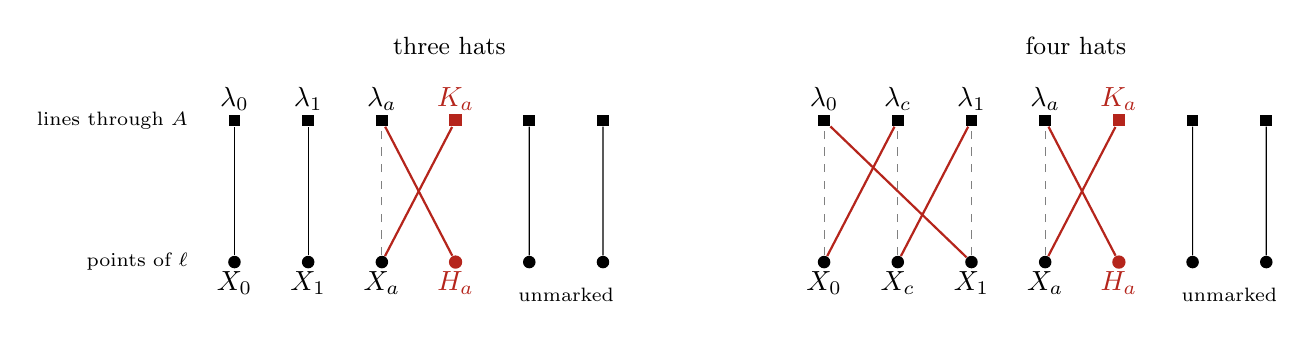
\begin{tikzpicture}[xscale=0.78,yscale=1.0]
\begin{scope}
  \node at (3.5,2.75) {\small three hats};
  \node[left,font=\scriptsize] at (-0.6,1.8) {lines through $A$};
  \node[left,font=\scriptsize] at (-0.6,0) {points of $\ell$};
  \foreach \x/\n/\l in {0/l0/\lam_0,1.2/l1/\lam_1,2.4/la/\lam_a,4.8/u1/{},6.0/u2/{}} {\node[ln] (\n) at (\x,1.8) {}; \node[above] at (\n) {$\l$};}
  \node[nln] (Ka) at (3.6,1.8) {}; \node[above] at (Ka) {\textcolor{BrickRed}{$K_a$}};
  \foreach \x/\n/\l in {0/X0/X_0,1.2/X1/X_1,2.4/Xa/X_a,4.8/Y1/{},6.0/Y2/{}} {\node[pt] (\n) at (\x,0) {}; \node[below] at (\n) {$\l$};}
  \node[npt] (Ha) at (3.6,0) {}; \node[below] at (Ha) {\textcolor{BrickRed}{$H_a$}};
  \node[font=\scriptsize] at (5.4,-0.42) {unmarked};
  \draw[old] (X0)--(l0); \draw[old] (X1)--(l1); \draw[old] (Y1)--(u1); \draw[old] (Y2)--(u2);
  \draw[gone] (Xa)--(la);
  \draw[added] (Xa)--(Ka); \draw[added] (Ha)--(la);
\end{scope}
\begin{scope}[xshift=9.6cm]
  \node at (4.1,2.75) {\small four hats};
  \foreach \x/\n/\l in {0/l0/\lam_0,1.2/lc/\lam_c,2.4/l1/\lam_1,3.6/la/\lam_a,6.0/u1/{},7.2/u2/{}} {\node[ln] (\n) at (\x,1.8) {}; \node[above] at (\n) {$\l$};}
  \node[nln] (Ka) at (4.8,1.8) {}; \node[above] at (Ka) {\textcolor{BrickRed}{$K_a$}};
  \foreach \x/\n/\l in {0/X0/X_0,1.2/Xc/X_c,2.4/X1/X_1,3.6/Xa/X_a,6.0/Y1/{},7.2/Y2/{}} {\node[pt] (\n) at (\x,0) {}; \node[below] at (\n) {$\l$};}
  \node[npt] (Ha) at (4.8,0) {}; \node[below] at (Ha) {\textcolor{BrickRed}{$H_a$}};
  \node[font=\scriptsize] at (6.6,-0.42) {unmarked};
  \draw[old] (Y1)--(u1); \draw[old] (Y2)--(u2);
  \draw[gone] (X0)--(l0); \draw[gone] (Xc)--(lc); \draw[gone] (X1)--(l1); \draw[gone] (Xa)--(la);
  \draw[added] (X0)--(lc); \draw[added] (Xc)--(l1); \draw[added] (X1)--(l0);
  \draw[added] (Xa)--(Ka); \draw[added] (Ha)--(la);
\end{scope}
\end{tikzpicture}
\caption{The incidences between the points of $\ell$ and the lines through $A$ (squares are lines, circles points; black: kept flags of $\Pi$, dashed: deleted flags, red: new). In $\Pi$ they form a perfect matching, $X\leftrightarrow AX$. In $\cS$ they still form a perfect matching, once the new point $H_a$ (which lies on $\ell$) is counted among the points of $\ell$ and the new line $K_a$ (which passes through $A$) among the lines through $A$: $X_a$ is now matched with $K_a$ and $\lam_a$ with $H_a$. The three hats keep the other flags. The four hats replace the three flags $(X_t,\lam_t)$, $t\in T$, by the cyclic shift $(X_t,\lam_{\sigma(t)})$, the \emph{rotation}. There are no other incidences between these points and lines.}
\label{fig:frame}
\end{figure}

\subsection{What the new elements are: a crossed doubling of the frame}\label{ssec:doubling}
The hat point $H_s$ is a copy of $X_s$ that does not see $\ell$; the hat line $K_s$ is a copy of $\lam_s$ that does not see $A$; and $(Q,M)$ is a copy of the anti-flag $(A,\ell)$ that does not see the elements $X_t$, $\lam_t$, $t\in T$. The cleanest way to say this is as a doubling of the frame, in the sense of Delorme \cite{D85a}, with one twist.

Let $\cF$ be the set of frame elements $A$, $\ell$, $X_s$, $\lam_s$ ($s\in S$), and give each $x\in\cF$ a copy $x'$ of the same kind:
\[
A'=Q,\qquad \ell'=M,\qquad X_s'=H_s,\qquad \lam_s'=K_s .
\]
The \emph{crossed doubling} $\cD$ of the frame has the points and lines of $\Pi$ and these copies, and the following incidences: all incidences of $\Pi$; for $x\in\cF$ and $y\notin\cF$ with $x\I y$, the incidence $x'\I y$ (a copy sees the same elements outside the frame as its original); for $x,y\in\cF$ with $x\I y$, the incidence $x'\I y'$ (copies see copies), except that each flag $(X_s,\lam_s)$ is \emph{crossed}: instead of $X_s'\I\lam_s'$ we put $X_s'\I\lam_s$ and $X_s\I\lam_s'$.

Reading off the neighbours of the copies: $H_s$ lies on $M$ (as $X_s\I\ell$) and on the lines through $X_s$ other than $\ell$ (those other than $\lam_s$ are outside $\cF$; $\lam_s$ by the crossing); $K_s$ contains $Q$ and the points of $\lam_s$ other than $A$; $M$ contains the hat points and the unmarked points of $\ell$; $Q$ lies on the hat lines and the lines through $A$ other than the $\lam_s$. Comparing with Definition~\ref{def:hats}:

\begin{proposition}\label{prop:doubling}
$\cS$ is obtained from the crossed doubling $\cD$ of the frame by
\begin{enumerate}[label=\textup{(\roman*)},leftmargin=2.5em]
\item adding the \emph{patches} $X_a\I M$, $Q\I\lam_a$, $A\I K_a$, $H_a\I\ell$ and $H_t\I K_{\pi(t)}$ \textup{(}$t\in T$\textup{)};
\item deleting the flags $(X_s,\lam_s)$, $s\in S$, and adding the flags $(X_t,\lam_{\rho(t)})$, $t\in T$ \textup{(}for the three hats: deleting $(X_a,\lam_a)$\textup{)}.
\end{enumerate}
\end{proposition}

So the question ``what happens to the combinatorics when these points and lines are added'' splits into two: what the doubling does (Lemma~\ref{lem:dbl}), and what the patches, the deletions and the rotation do (\S\ref{ssec:patches}).

\begin{lemma}\label{lem:dbl}
Suppose $\ell$ has an unmarked point \textup{(}$|S|\le q$\textup{)}. In the crossed doubling $\cD$:
\begin{enumerate}[label=\textup{(\alph*)}]
\item $X_s$ and $\lam_s$ have degree $q+2$; $A$, $\ell$, $Q$, $M$, $H_s$, $K_s$ have degree $q+1$; an element outside $\cF$ has degree $q+2$ if it is on $\ell$ or on some $\lam_s$ \textup{(}a point\textup{)}, or passes through $A$ or some $X_s$ \textup{(}a line\textup{)}, and degree $q+1$ otherwise.
\item The pairs of points that are not collinear are exactly
\[
\{H_s,X_t\}\ (s\ne t)\qquad\text{and}\qquad\{H_s,Q\},
\]
and the pairs of lines that are not concurrent are exactly $\{K_s,\lam_t\}$ \textup{(}$s\ne t$\textup{)} and $\{K_s,M\}$.
\end{enumerate}
\end{lemma}

\begin{proof}
(a) $X_s$ gains $K_s$ (crossing) and $\lam_s$ gains $H_s$; $A$ and $\ell$ gain nothing, since their frame neighbours are copied together with them. $Q$ lies on $|S|$ hat lines and $q+1-|S|$ lines through $A$; $H_s$ on $M$ and $q$ lines; dually for $M$, $K_s$. A point outside $\cF$ gains $M$ if it is on $\ell$ and $K_s$ if it is on $\lam_s$ (at most one of these, as it is not $A$ or an $X_s$).

(b) Two points of $\Pi$ keep their common line. $Q$ and a point $u$ of $\Pi$: if $u=A$, use a line through $A$ outside $\cF$ (there is one, as $|S|\le q$; for the four hats with $q=3$ there is none, and $\{Q,A\}$, $\{M,\ell\}$ are two more far pairs, repaired by the patches $Q\I\lam_a$ and $X_a\I M$); if $Au$ is not a $\lam_s$, use $Au$; if $u\neq A$ is on $\lam_s$, use $K_s$. $H_s$ and a point $u\notin\ell$: use $uX_s$, which is not $\ell$. $H_s$ and $X_s$: a line through $X_s$ outside $\cF$. $H_s$ and an unmarked point of $\ell$: $M$. Two hat points: $M$. This leaves $H_s$ and $X_t$ ($t\ne s$), whose only common line in $\Pi$ is $\ell$, which $H_s$ is not on, while $M\not\ni X_t$ and the other lines of $H_s$ meet $\ell$ only in $X_s$; and $H_s$ and $Q$, which have no common line ($Q$ is on no line through $X_s$ except possibly $\lam_s$, and $Q\notin\lam_s$; $Q\notin M$). The statement for lines is the same argument with points and lines exchanged; $\cD$ is built from $\Pi$ and the frame by rules that are symmetric under this exchange.
\end{proof}

So the copies cost nothing among the old points: no two points of $\Pi$ become non-collinear and no two lines of $\Pi$ stop meeting. The failures all involve a copy, and they come from paths of length $2$ inside the frame: $X_s-\ell-X_t$ (the copy $H_s$ of $X_s$ does not see $\ell$, and the original $X_t$ does not see the copy $M$ of $\ell$) and $X_s-\lam_s-A$ (the crossing removes the copy $H_s-K_s-Q$ of this path). For Delorme's doubling without crossing, the hat lemma (\path{POLISHED.md}, Lemma~1.3) says that a set of elements of a projective plane can be doubled without changing the diameter only if each of its connected components is a single element or a flag; the frame contains the paths $\ell,X_s,\lam_s,A$, so some patching is unavoidable. Lemma~\ref{lem:dbl}(a) also says that the doubling leaves exactly one free incidence at each of the $2|S|+4$ elements $A,\ell,Q,M,H_s,K_s$, and none at $X_s$, $\lam_s$.

\subsection{The patches, the deletions and the rotation}\label{ssec:patches}
The patches of Proposition~\ref{prop:doubling}(i) spend the free incidences of $A,\ell,Q,M,H_s,K_s$, one each. The far pairs of Lemma~\ref{lem:dbl}(b) are repaired as follows (a pair $\{H_s,X_t\}$ always has $s\neq t$):

\begin{center}\small
\renewcommand{\arraystretch}{1.15}
\begin{tabular}{@{}lll@{}}
\toprule
far pair in $\cD$ & common line in $\cS$ & because of\\
\midrule
$\{H_s,X_a\}$ & $M$ & patch $X_a\I M$\\
$\{H_a,X_t\}$ & $\ell$ & patch $H_a\I\ell$\\
$\{H_t,X_{\pi(t)}\}$, $t\in T$ & $K_{\pi(t)}$ & link $H_t\I K_{\pi(t)}$ (and $X_{\pi(t)}\I K_{\pi(t)}$)\\
$\{H_t,X_{\sigma^{-1}(t)}\}$, $t\in T$ (four hats) & $\lam_t$ & rotation $X_{\sigma^{-1}(t)}\I\lam_t$ (and $H_t\I\lam_t$)\\
$\{H_a,Q\}$ & $\lam_a$ & patch $Q\I\lam_a$ (and $H_a\I\lam_a$)\\
$\{H_t,Q\}$, $t\in T$ & $K_{\pi(t)}$ & link $H_t\I K_{\pi(t)}$\\
\bottomrule
\end{tabular}
\end{center}

\noindent The far pairs of lines are repaired dually: $\{K_s,\lam_a\}$ by $Q$, $\{K_a,\lam_t\}$ by $A$, $\{K_{\pi(t)},\lam_t\}$ by $H_t$, $\{K_t,\lam_{\sigma(t)}\}$ by $X_t$ (four hats), $\{K_a,M\}$ by $X_a$, $\{K_{\pi(t)},M\}$ by $H_t$.

\emph{Why the three hats need no rotation and the four hats do.} The pairs $\{H_s,X_t\}$ with $s=a$ or $t=a$ are repaired by $\ell$ and $M$. What remains is $\{H_t,X_u\}$ for $t\ne u$ in $T$: each hat point $H_t$ must reach the $|T|-1$ points $X_u$, $u\in T\setminus\{t\}$, and it has one free incidence, which goes to a link. For the three hats $|T|-1=1$ and the link $H_t\I K_{\pi(t)}$ suffices. For the four hats $|T|-1=2$: the link reaches $X_{\sigma(t)}$, and $X_{\sigma^{-1}(t)}$ is reached through $\lam_t$, which already carries $H_t$, after the rotation has moved $X_{\sigma^{-1}(t)}$ onto $\lam_t$. Hence $\rho=\pi=\sigma$: $\rho^{-1}(t)$ must be the element of $T\setminus\{t\}$ that $\pi$ does not reach. (Dually each hat line $K_t$ meets $\lam_{\sigma(t)}$ in $X_t$ and $\lam_{\sigma^{-1}(t)}$ in $H_{\sigma^{-1}(t)}$.) With $|T|=4$ the same count gives a hat point two ways to reach three points, which is one heuristic reason why the pattern stops at four hats; a SAT search confirms that no fifth hat can be added inside this family for $q=4,5,7,8,9,11,13$ (\path{research/plus2/REPORT.md}).

\emph{Why the flags $(X_s,\lam_s)$ are deleted.} The patches $X_a\I M$ and $Q\I\lam_a$ raise the degrees of $X_a$ and $\lam_a$, which were already $q+2$, to $q+3$; deleting the flag $(X_a,\lam_a)$ brings both back to $q+2$. The rotation is degree-neutral: $X_t$ trades $\lam_t$ for $\lam_{\sigma(t)}$, and $\lam_t$ trades $X_t$ for $X_{\sigma^{-1}(t)}$. Deleting a flag $(X,\lam)$ from a projective plane makes exactly $q$ pairs of points non-collinear (the pairs $\{X,Y\}$, $Y$ a point of $\lam$ other than $X$) and $q$ pairs of lines non-concurrent (the pairs $\{\lam,N\}$, $N$ a line through $X$ other than $\lam$). After the deletions and the rotation, the pairs of points of $\Pi$ that have no common line of $\Pi$ any more are:
\begin{itemize}[leftmargin=1.5em]
\item three hats: $\{X_a,Y\}$ for the $q$ points $Y\ne X_a$ of $\lam_a$, and dually $\{\lam_a,N\}$ for the $q$ lines $N\neq\lam_a$ through $X_a$;
\item four hats: $\{X_s,Y\}$ for $s\in S$ and the $q-1$ points $Y$ of $\lam_s$ other than $A$ and $X_s$, and $\{X_a,A\}$; dually $\{\lam_s,N\}$ for the $q-1$ lines $N$ through $X_s$ other than $\ell$ and $\lam_s$, and $\{\lam_a,\ell\}$. That is $4(q-1)+1$ pairs of each kind. The pairs $\{X_t,A\}$ and $\{\lam_t,\ell\}$, $t\in T$, are not broken, because $X_t$ and $A$ are both on $\lam_{\sigma(t)}$, and $\lam_t$ and $\ell$ both contain $X_{\sigma^{-1}(t)}$.
\end{itemize}
Each broken pair is repaired by the crossing and one patch: $X_s$ and the points of $\lam_s$ other than $A$ are all on $K_s$ (rule~\ref{r:hatline}), and $A\I K_a$ repairs $\{X_a,A\}$; dually $\lam_s$ and the lines through $X_s$ other than $\ell$ all pass through $H_s$, and $H_a\I\ell$ repairs $\{\lam_a,\ell\}$. This is why the flags may be deleted at all: the crossing has already given every point of $\lam_s$ a second line through $X_s$ (namely $K_s$), and every line through $X_s$ a second point on $\lam_s$ (namely $H_s$).

Figure~\ref{fig:hatpair} shows the local picture at a hat pair; Table~\ref{tab:gadget} shows the whole gadget.

\begin{figure}[ht]
\centering
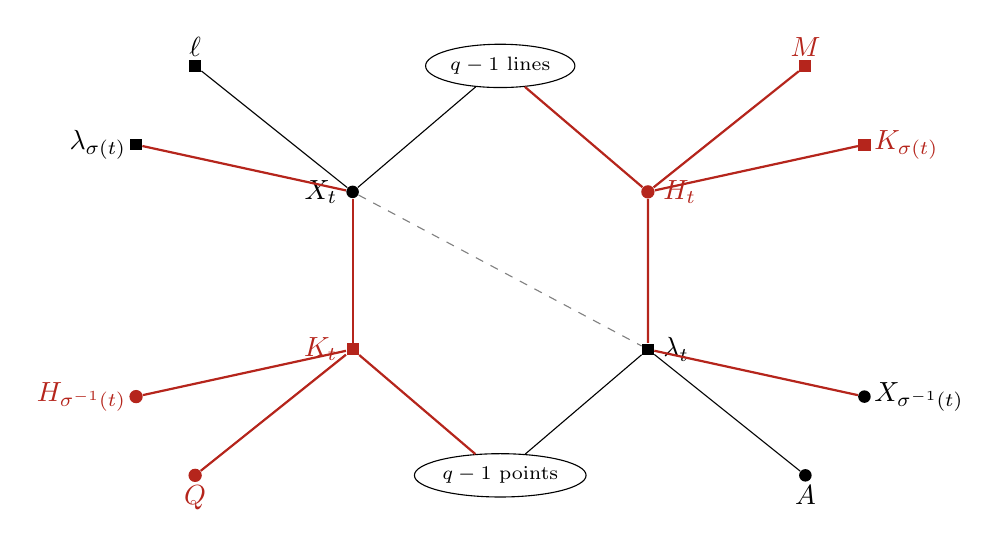
\begin{tikzpicture}[xscale=1.25,yscale=1.0]
  \node[pt] (X) at (0,2) {}; \node[left=2pt] at (X) {$X_t$};
  \node[npt] (H) at (3,2) {}; \node[right=2pt] at (H) {\textcolor{BrickRed}{$H_t$}};
  \node[nln] (K) at (0,0) {}; \node[left=2pt] at (K) {\textcolor{BrickRed}{$K_t$}};
  \node[ln] (L) at (3,0) {}; \node[right=2pt] at (L) {$\lam_t$};
  \node[blob] (N) at (1.5,3.6) {$q-1$ lines};
  \node[blob] (Y) at (1.5,-1.6) {$q-1$ points};
  \node[ln] (ell) at (-1.6,3.6) {}; \node[above] at (ell) {$\ell$};
  \node[ln] (lsig) at (-2.2,2.6) {}; \node[left] at (lsig) {$\lam_{\sigma(t)}$};
  \node[nln] (M) at (4.6,3.6) {}; \node[above] at (M) {\textcolor{BrickRed}{$M$}};
  \node[nln] (Ksig) at (5.2,2.6) {}; \node[right] at (Ksig) {\textcolor{BrickRed}{$K_{\sigma(t)}$}};
  \node[pt] (A) at (4.6,-1.6) {}; \node[below] at (A) {$A$};
  \node[pt] (Xsig) at (5.2,-0.6) {}; \node[right] at (Xsig) {$X_{\sigma^{-1}(t)}$};
  \node[npt] (Q) at (-1.6,-1.6) {}; \node[below] at (Q) {\textcolor{BrickRed}{$Q$}};
  \node[npt] (Hsig) at (-2.2,-0.6) {}; \node[left] at (Hsig) {\textcolor{BrickRed}{$H_{\sigma^{-1}(t)}$}};
  \draw[old] (X)--(N); \draw[added] (H)--(N);
  \draw[old] (L)--(Y); \draw[added] (K)--(Y);
  \draw[added] (X)--(K); \draw[added] (H)--(L);
  \draw[gone] (X)--(L);
  \draw[old] (X)--(ell); \draw[added] (X)--(lsig);
  \draw[added] (H)--(M); \draw[added] (H)--(Ksig);
  \draw[old] (L)--(A); \draw[added] (L)--(Xsig);
  \draw[added] (K)--(Q); \draw[added] (K)--(Hsig);
\end{tikzpicture}
\caption{The local picture at a hat pair $(H_t,K_t)$, $t\in T$, of the four hats, in the incidence graph. Circles are points, squares are lines, new elements and new incidences are red, the dashed edge is the deleted flag $(X_t,\lam_t)$. The upper blob is the set of $q-1$ lines through $X_t$ other than $\ell$ and $\lam_t$, the lower blob the $q-1$ points of $\lam_t$ other than $A$ and $X_t$. $H_t$ and $X_t$ are twins on the upper blob, $K_t$ and $\lam_t$ twins on the lower blob, and the flag $(X_t,\lam_t)$ is replaced by the crossed pair $X_t\I K_t$, $H_t\I\lam_t$. Every element shown has degree $q+2$. For the three hats ($t\in\{0,1\}$) the dashed flag is kept, the edges to $\lam_{\sigma(t)}$ and $X_{\sigma^{-1}(t)}$ are absent, and the links go to $K_{\pi(t)}$ and $H_{\pi(t)}$, $\pi=(0\ 1)$.}
\label{fig:hatpair}
\end{figure}

\subsection{Degrees and counts}\label{ssec:degrees}

\begin{lemma}\label{lem:deg}
In $\cS$ every element has degree $q+1$ or $q+2$. The points of degree $q+1$ \textup{(}the \emph{deficient} points\textup{)} are the points of $\Pi$ off $\ell$, other than $A$, on the lines joining $A$ to the unmarked points of $\ell$; dually, the lines of degree $q+1$ are the lines of $\Pi$ not through $A$, other than $\ell$, through the unmarked points of $\ell$. There are $(q-1)(q+1-|S|)$ of each: $(q-1)(q-2)$ for the three hats and $(q-1)(q-3)$ for the four hats. Each deficient point lies on exactly $q-|S|$ deficient lines, and each deficient line has exactly $q-|S|$ deficient points.
\end{lemma}

\begin{proof}
Count the lines through each point: those of $\Pi$, minus deleted flags, plus added ones. $A$: $q+1$ lines and $K_a$. An unmarked point of $\ell$: $q+1$ lines and $M$. $X_a$: loses $\lam_a$, gains $M$ and $K_a$. $X_t$, $t\in T$: four hats, loses $\lam_t$ and gains $\lam_{\sigma(t)}$ and $K_t$; three hats, gains $K_t$. A point $p\notin\ell$, $p\neq A$: it is on exactly one line through $A$, the line $Ap$; it loses nothing, and gains $K_s$ exactly when $Ap=\lam_s$. $Q$: $|\Lambda^*|+|S|=(q+1-|T|)+|S|=q+2$. $H_s$: $q$ lines by~\ref{r:hat}, $M$, and one link line. The lines are the dual count (Lemma~\ref{lem:dual} below). A deficient point $p$ lies on $Ap$ and on $q$ lines meeting $\ell$ in the $q$ points other than $Ap\cap\ell$; among these, $q-|S|$ are unmarked.
\end{proof}

So $\cS$ has $q^2+q+1+|S|+1$ points and as many lines: $2(q^2+q+5)$ elements for the three hats and $2(q^2+q+6)$ for the four hats. To make it regular, join each deficient point to a deficient line not through it, by a perfect matching. Such a matching exists when there are deficient elements ($|S|\le q$; for the four hats with $q=3$ the structure is already regular): the bipartite graph of non-incident pairs between deficient points and deficient lines is regular of degree $(q-1)(q+1-|S|)-(q-|S|)>0$, and a regular bipartite graph of positive degree has a perfect matching (K\"onig). Adding flags cannot increase distances. (In $\mathrm{PG}(2,q)$ explicit matchings are given in coordinates in \cite{AL20} and in \path{coords.tex}; any matching of non-incident pairs works.)

\subsection{The diameter}\label{ssec:diam}

\begin{lemma}[Points]\label{lem:points}
Any two distinct points of $\cS$ are collinear in $\cS$; Table~\ref{tab:cases} gives a common line for every pair.
\end{lemma}

\begin{table}[ht]
\centering\small
\renewcommand{\arraystretch}{1.18}
\begin{tabular}{@{}>{\raggedright}p{0.52\textwidth}>{\raggedright}p{0.2\textwidth}>{\raggedright\arraybackslash}p{0.2\textwidth}@{}}
\toprule
pair of points & common line & three hats\\
\midrule
\multicolumn{3}{@{}l}{\emph{two points $u,v$ of $\Pi$}}\\
the line $uv$ of $\Pi$ keeps both incidences & $uv$ & \\
$u=X_s$, $v$ a point of $\lam_s$ other than $A$, $X_s$, flag $(X_s,\lam_s)$ deleted & $K_s$ & only $s=a$\\
$u=X_a$, $v=A$ & $K_a$ & \\
$u=X_t$, $v=A$, $t\in T$ (four hats) & $\lam_{\sigma(t)}$ & $\lam_t$ is kept\\
\multicolumn{3}{@{}l}{\emph{$Q$ and a point $u$ of $\Pi$}}\\
$u=A$ & $\lam_a$ & \\
$u=X_s$ & $K_s$ & \\
$u$ an unmarked point of $\ell$ & $Au$ & \\
$u\notin\ell$, $u\ne A$, $Au\in\Lambda^*$ & $Au$ & \\
$u\notin\ell$, $u\ne A$, $Au=\lam_t$ with $t\in T$ & $K_t$ & \\
\multicolumn{3}{@{}l}{\emph{$H_s$ and a point $u$ of $\Pi$}}\\
$u\notin\ell$ (including $u=A$) & $uX_s$ & \\
$u=X_s$ & a line through $X_s$ other than $\ell,\lam_s$ & \\
$u\in\ell^*$, $u\neq X_s$ & $M$ & \\
$s=a$, $u=X_t$ with $t\in T$ & $\ell$ & \\
$s=t\in T$, $u=X_{\pi(t)}$ & $K_{\pi(t)}$ & $\pi=(0\ 1)$\\
$s=t\in T$, $u=X_{\sigma^{-1}(t)}$ (four hats) & $\lam_t$ & does not occur\\
\multicolumn{3}{@{}l}{\emph{two new points}}\\
$H_s$ and $H_{s'}$ & $M$ & \\
$Q$ and $H_a$ & $\lam_a$ & \\
$Q$ and $H_t$, $t\in T$ & $K_{\pi(t)}$ & \\
\bottomrule
\end{tabular}
\caption{A common line for every pair of distinct points of $\cS$. Here $s,s'\in S$ and $t\in T$. The third column notes where the three hats differ; elsewhere the entry is the same for both constructions.}
\label{tab:cases}
\end{table}

\begin{proof}
We check that Table~\ref{tab:cases} covers every pair and that each named line contains both points. The only flags of $\Pi$ missing from $\cS$ are among the $(X_s,\lam_s)$; so a flag $(u,L)$ of $\Pi$ survives whenever $u\notin\ell$ or $L$ does not pass through $A$.

\emph{Two points of $\Pi$.} If the line $uv$ of $\Pi$ lost an incidence, then (up to order) $u=X_s$, $uv=\lam_s$ with the flag deleted, and $v$ is $A$ or another point of $\lam_s$. If $v\neq A$, both lie on $K_s$ by~\ref{r:hatline}. If $v=A$ and $s=a$: $X_a\I K_a$ by~\ref{r:hatline} and $A\I K_a$ by~\ref{r:links}. If $v=A$ and $s=t\in T$ (four hats): the rotation puts $X_t$ on $\lam_{\sigma(t)}$, which passes through $A$.

\emph{$Q$ and a point $u$ of $\Pi$.} $\lam_a\in\Lambda^*$ passes through $A$ and carries $Q$. $K_s$ contains $X_s$ and $Q$. An unmarked point $u$ of $\ell$: $Au\in\Lambda^*$, and the flag $(u,Au)$ was not touched. A point $u\notin\ell$, $u\ne A$: the flag $(u,Au)$ survives; if $Au\in\Lambda^*$ it carries $Q$; otherwise $Au=\lam_t$, $t\in T$, and $u$ is a point of $\lam_t$ other than $A$, so $u\I K_t\ni Q$.

\emph{$H_s$ and a point $u$ of $\Pi$.} If $u\notin\ell$, the line $uX_s$ of $\Pi$ is not $\ell$, so it carries $H_s$, and it contains $u$ in $\cS$. If $u=X_s$, any of the $q-1\ge1$ lines through $X_s$ other than $\ell$ and $\lam_s$ carries both. If $u\in\ell^*$ (this includes $X_a$ when $s\neq a$), use $M$. The remaining case is $u=X_{t'}$ with $t'\in T\setminus\{s\}$. If $s=a$, then $H_a\I\ell$. If $s=t\in T$: for the three hats $t'=\pi(t)$; for the four hats $t'\in\{\sigma(t),\sigma^{-1}(t)\}$, as $\sigma$ is a $3$-cycle. The line $K_{\pi(t)}$ contains $X_{\pi(t)}$ by~\ref{r:hatline} and $H_t$ by the link. The line $\lam_t$ contains $X_{\sigma^{-1}(t)}$ by the rotation and $H_t$ by~\ref{r:hat}.

\emph{Two new points.} $M$ carries all hat points. $\lam_a$ carries $Q$ (as $\lam_a\in\Lambda^*$) and $H_a$ (as a line through $X_a$ other than $\ell$). $K_{\pi(t)}$ carries $Q$ and, by the link, $H_t$.
\end{proof}

For lines we use duality. In the dual plane $\Pi^D$ the line $\ell$ is a point and $A$ a line not through it, the lines $\lam_s$ are points on the line $A$, and the line joining the points $\ell$ and $\lam_s$ is the point $X_s$.

\begin{lemma}[Duality]\label{lem:dual}
The dual of $\cS(\Pi;A,\ell,(X_s),\pi,\rho)$ is $\cS(\Pi^D;\ell,A,(\lam_s),\pi^{-1},\rho^{-1})$, by the identity on the elements of $\Pi$ and $H_s\leftrightarrow K_s$, $Q\leftrightarrow M$. Consequently any two distinct lines of $\cS$ are concurrent.
\end{lemma}

\begin{proof}
Read the six rules in $\Pi^D$ with the frame $(\ell,A,(\lam_s))$. Rule~\ref{r:plane} deletes the flags $(\lam_s,X_s)$ and adds $\lam_t\I X_{\rho^{-1}(t)}$, which is the rotation $X_u\I\lam_{\rho(u)}$ of $\cS$. Rule~\ref{r:hat} gives a new element incident with every element incident with $\lam_s$ other than $A$: this is $K_s$; rule~\ref{r:hatline} gives one incident with every element incident with $X_s$ other than $\ell$: this is $H_s$. Rule~\ref{r:M} gives a new element incident with the lines through $A$ other than the $\lam_t$, $t\in T$, and with all $K_s$: this is $Q$; likewise~\ref{r:Q} gives $M$. Rule~\ref{r:links} gives $\ell\I H_a$, $K_a\I A$ and $K_t\I H_{\pi^{-1}(t)}$, which are the links of $\cS$. Since $\Pi^D$ is a projective plane of order $q$ and $\pi^{-1}$, $\rho^{-1}$ are again of the required kind (for the three hats $\pi^{-1}=\pi$, $\rho^{-1}=\rho$; for the four hats $\pi^{-1}=\rho^{-1}=\sigma^{-1}$, a $3$-cycle), Lemma~\ref{lem:points} for the dual structure says that any two lines of $\cS$ are concurrent.
\end{proof}

\begin{theorem}\label{thm:hats}
Let $\Pi$ be a projective plane of order $q\ge 3$. The three-hat structure of \cite{AL20} and the four-hat structure are incidence structures with all degrees $q+1$ or $q+2$ and diameter $3$, with $2(q^2+q+5)$ and $2(q^2+q+6)$ elements. Adding a perfect matching of non-incident pairs between the deficient points and lines makes them $(q+2)$-regular. Hence $n_b(q+2,3)\ge 2(q^2+q+6)$ for every prime power $q\ge 3$.
\end{theorem}

\begin{proof}
Degrees and counts are Lemma~\ref{lem:deg}. Every element is incident with something. By Lemmas~\ref{lem:points} and~\ref{lem:dual} any two points are collinear and any two lines concurrent, so by Lemma~\ref{lem:diam}(a) the diameter is at most $3$; it is $3$ because $A\nI\ell$.
\end{proof}

Only the axioms of a projective plane are used, so the theorem holds in non-Desarguesian planes too (we checked the nearfield plane of order $9$). In the range of the tables, $q=9,11,13$ give $192$, $276$, $376$ at $\Delta=11,13,15$, two more than \cite{AL20}.

\subsection{From three hats to four, step by step}\label{ssec:steps}
Start from the three hats with labels $0,1,a$ and choose a fourth point $X_c$ of $\ell$, different from $X_0,X_1,X_a$. The four-hat structure arises by exactly these changes:
\begin{enumerate}[label=\textup{(\arabic*)},leftmargin=2.5em]
\item add the point $H_c$, on the $q$ lines through $X_c$ other than $\ell$, on $M$ and on $K_1$; add the line $K_c$, through the $q$ points of $\lam_c$ other than $A$, through $Q$ and through $H_0$;
\item delete the flags $(X_0,\lam_0)$, $(X_c,\lam_c)$, $(X_1,\lam_1)$, and add $(X_0,\lam_c)$, $(X_c,\lam_1)$, $(X_1,\lam_0)$;
\item delete $X_c\I M$ and $Q\I\lam_c$ (now $X_c$ is a $T$-point and $\lam_c$ a $T$-line);
\item delete the link $H_0\I K_1$; it is replaced by $H_0\I K_c$ and $H_c\I K_1$ from (1), while $H_1\I K_0$ is kept.
\end{enumerate}
In terms of the links, the cycle $0\to1\to0$ of $\pi=(0\ 1)$ becomes the cycle $0\to c\to 1\to 0$ of $\sigma$. The four-hat structure has $2q+1$ more flags than the three-hat structure: $2(q+2)$ at $H_c$ and $K_c$, three from the rotation, minus six. (Checked by computer against the coordinate versions for $q=4,5,7$ and every choice of $a,c$.)

\section{Diameter 4}\label{sec:d4}
\emph{To be written.}

\section{Diameter 6}\label{sec:d6}
\emph{To be written.}

\section{Diameter 7}\label{sec:d7}
\emph{To be written.}

\appendix
\section{Coordinates and checks}\label{app:checks}
Explicit coordinates for every construction: \path{POLISHED.md} (\S2 for the hats, \S\S3--5 for diameter $4$, \S\S6--7 for diameter $6$) and \path{D7_HEXAGON.md} (diameter $7$). The check script for Section~\ref{sec:d3} is \path{research/synthetic/checks/check_d3.py}; its output is in \path{check_d3.out}.

\begin{thebibliography}{99}
\bibitem{AL20} G.~Araujo-Pardo and N.~L\'opez, On new record graphs close to bipartite Moore graphs, Graphs Combin. \textbf{38} (2022), no.~4, Paper 110; arXiv:2005.02427.
\bibitem{D85a} C.~Delorme, Grands graphes de degr\'e et diam\`etre donn\'es, European J. Combin. \textbf{6} (1985), 291--302.
\end{thebibliography}

\end{document}
